\newtoggle{PAPERS}
\toggletrue{PAPERS}

\chapter{Results}

\todo[inline]{Consider promoting the paper sections to chapters.}

The results of my research have been published at a number of conferences and workshops.
This chapter includes a selection of these publications.
Each of the publications is self-contained.

\todo[inline]{In each section, summarize the results of the respective paper.}

\section{Learning Precedences from Simple Symbol Features}
\label{sec:results:simple}

Filip Bártek and Martin Suda. Learning Precedences from Simple Symbol Features. \Gls{paar} 2020. \cite{DBLP:conf/cade/Bartek020}

\todo[inline]{Consider removing this paper. Am I allowed to include it even though it's not prestigious?}

\iftoggle{PAPERS}{
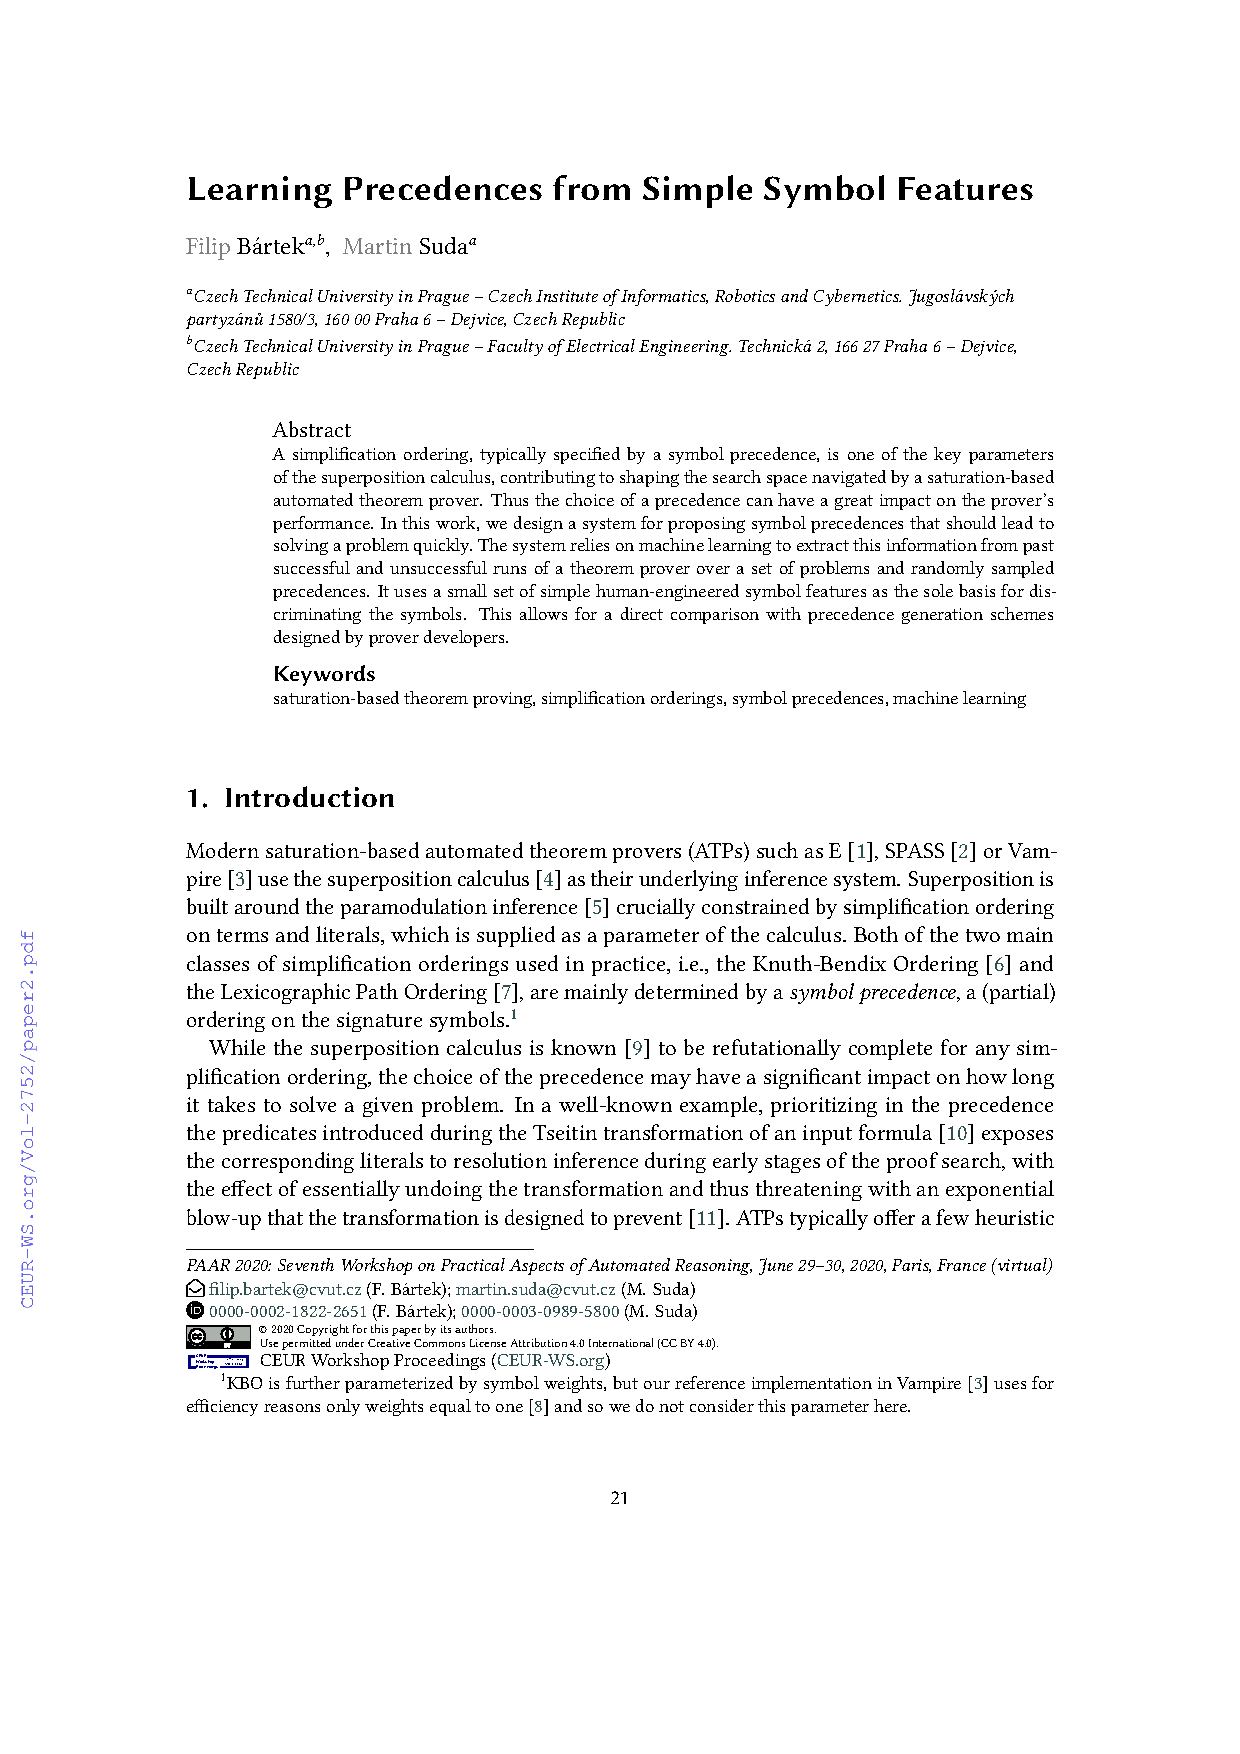
\includepdf[pages=-]{publications/simple.pdf}
}

\section{Neural Precedence Recommender}
\label{sec:results:npr}

Filip Bártek and Martin Suda. Neural Precedence Recommender. \Gls{cade} 28, 2021. \cite{DBLP:conf/cade/Bartek021}

\iftoggle{PAPERS}{
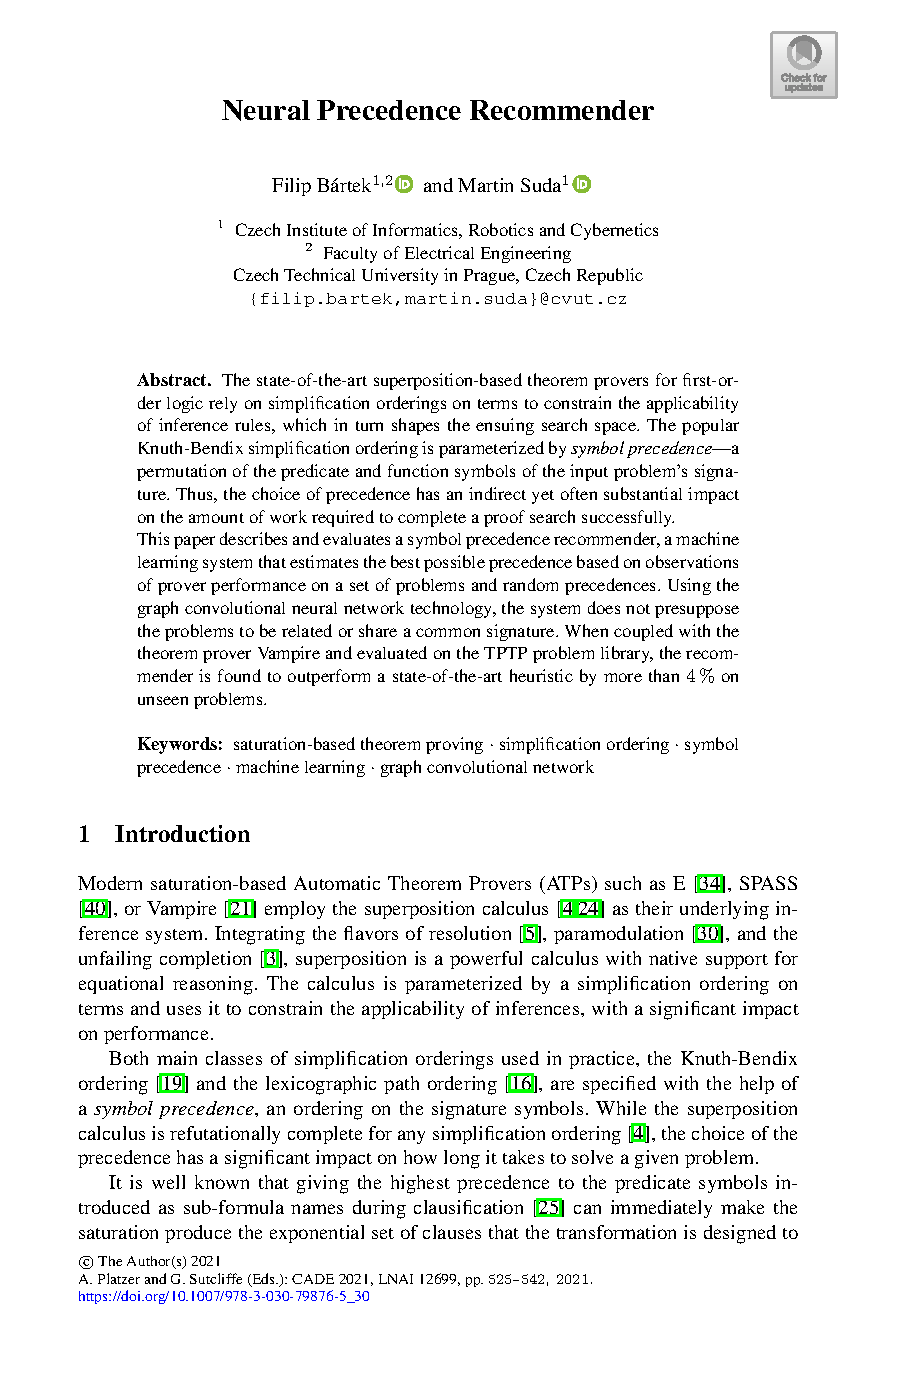
\includepdf[pages=-]{publications/Neural Precedence Recommender.pdf}
}

\section{A GNN-Advised Clause Selection}
\label{sec:results:selection}

Filip Bártek and Martin Suda. How much should this symbol weigh? A \acrshort{gnn}-Advised Clause Selection \cite{DBLP:conf/lpar/Bartek023}

\iftoggle{PAPERS}{
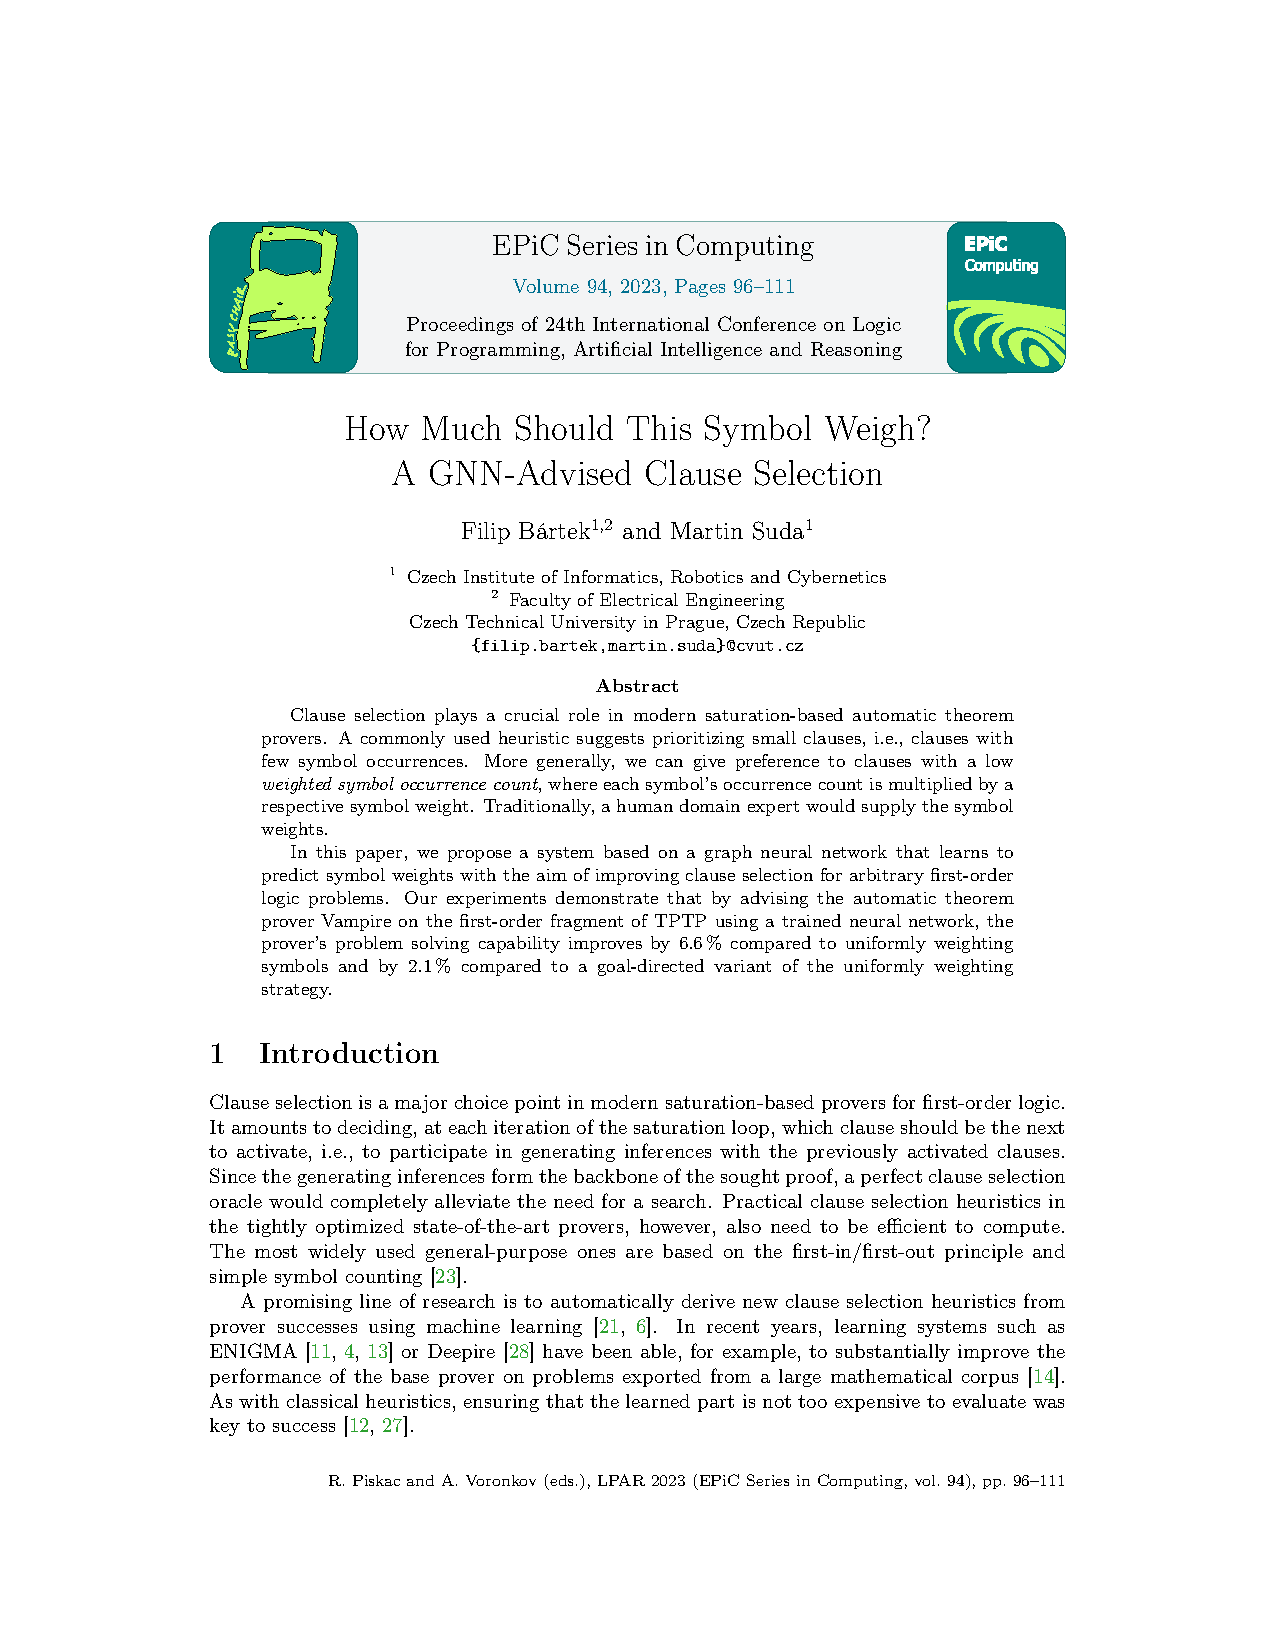
\includepdf[pages=-]{publications/weights.pdf}
}

\section{Regularization in Spider-Style Strategy Discovery and Schedule Construction}
\label{sec:results:regularization}

Filip Bártek, Karel Chvalovský, and Martin Suda. Regularization in Spider-Style Strategy Discovery and Schedule Construction. \Gls{ijcar}, 2024 (accepted). \cite{bartek2024regularization}\todo{Replace by the final version and link to the arXiv version with appendix.}

In this paper, we invented strong complementary strategies for the \gls{atper} Vampire and constructed strong schedules that generalize well.

\iftoggle{PAPERS}{
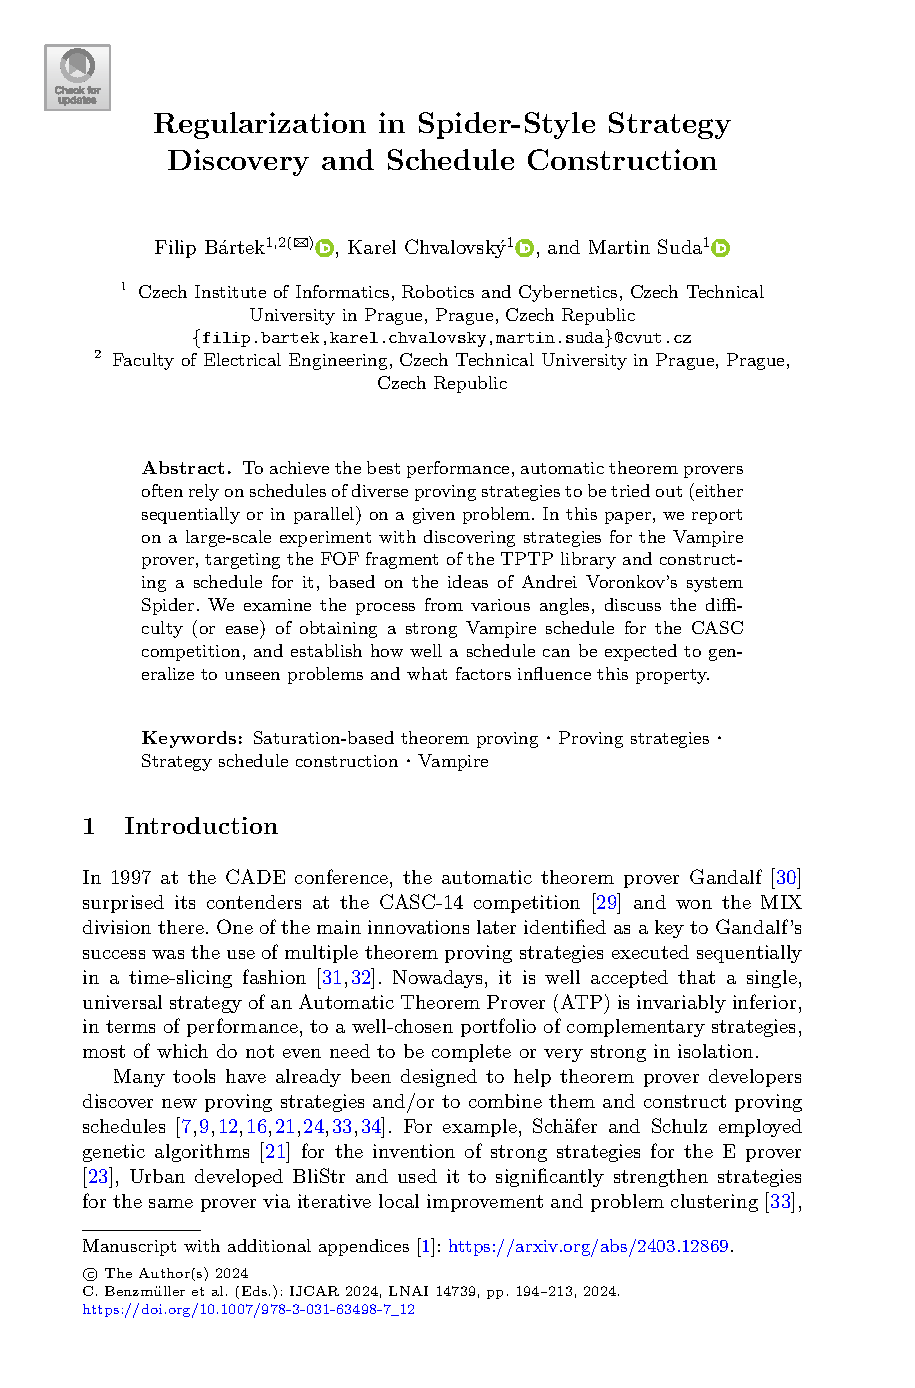
\includepdf[pages=-]{publications/regularization.pdf}
}

\todo[inline]{Consider including PAAR 2024 paper.}
